\section{Results}
\subsection{Track 1}
\begin{table}
  \caption{Leaderboard for Track T1. Recall achieved at 10000 QPS on Azure F32v2 VM with 32 vCPUs.}
  
  \begin{tabular}{l|c|c|c|c|c|c}
    \hline
    Algorithm & bigann-1B & deep-1B & msspacev-1B & msturing-1B & ssnpp-1B & text2image-1B  \\
    \hline
    Baseline  &	0.63451   & 0.65028 & 0.728861 & 0.703611 & 0.75378 & 0.069275       \\
    \hline
    \href{https://github.com/harsha-simhadri/big-ann-benchmarks/pull/58}{team11}     & & 0.64955 & & 0.712211 & & \\
    \href{https://github.com/harsha-simhadri/big-ann-benchmarks/pull/60}{puck-t1}    & 0.71468   & 0.72255 & & 0.793812* & & 0.160987*    \\
    \href{https://github.com/harsha-simhadri/big-ann-benchmarks/pull/66}{ngt-t1}     & & & & & & \\
    \href{https://github.com/harsha-simhadri/big-ann-benchmarks/pull/69}{kst\_ann\_t1} &	0.71219	  & 0.71219 & 0.764542 & 0.756419 & & \\
    \href{https://github.com/harsha-simhadri/big-ann-benchmarks/pull/71}{buddy-t1}   &	0.62765 & & & & \\
    \hline
  \end{tabular}
\end{table}


\begin{figure}[ht]
  \begin{subfigure}{0.48\textwidth}
    \centering
    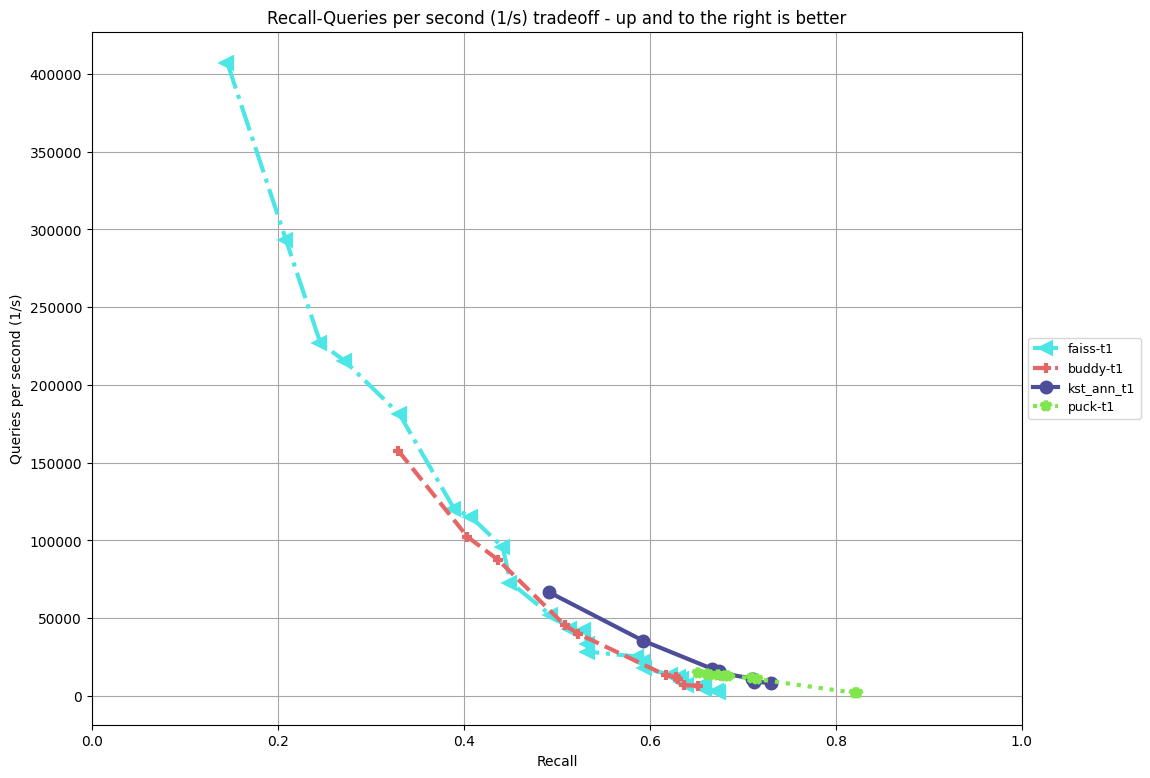
\includegraphics[width=\linewidth]{../t1_t2/results/T1/neurips21/bigann-1B.png}
      \caption{bigann-1B}
  \end{subfigure}
  \begin{subfigure}{0.48\textwidth}
    \centering
    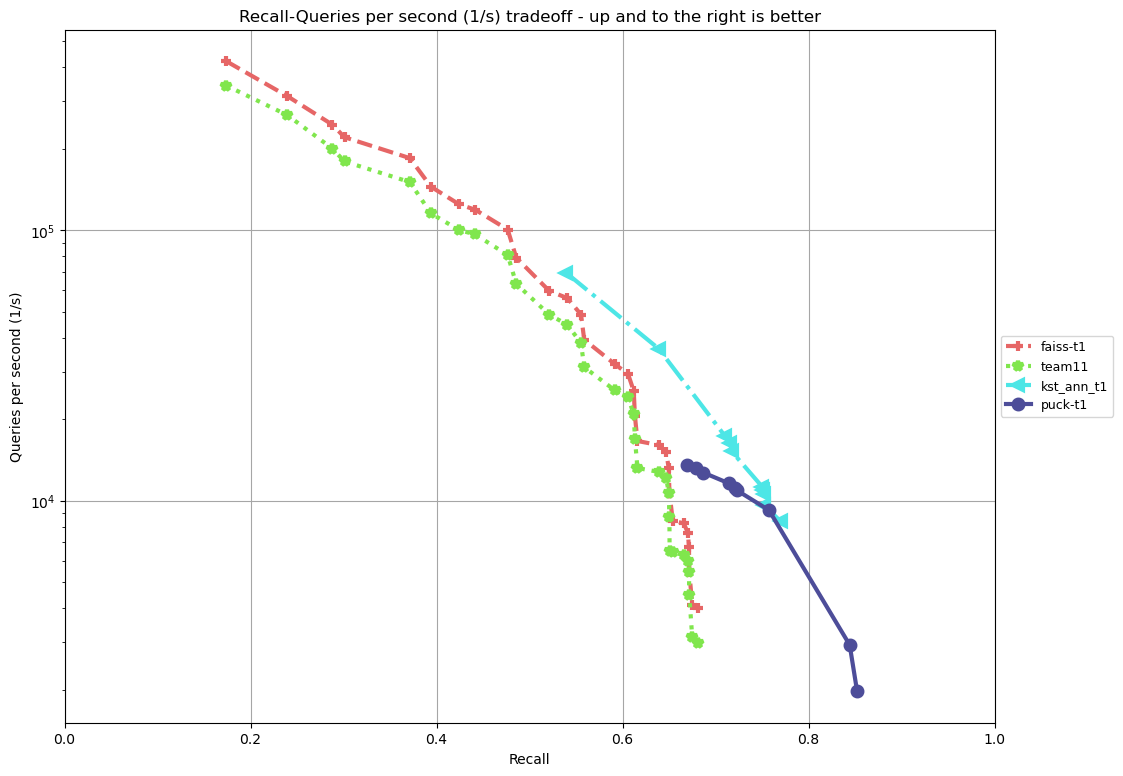
\includegraphics[width=\linewidth]{../t1_t2/results/T1/neurips21/deep-1B.png}
    \caption{deep-1B}
  \end{subfigure}
  \begin{subfigure}{0.48\textwidth}
    \centering
    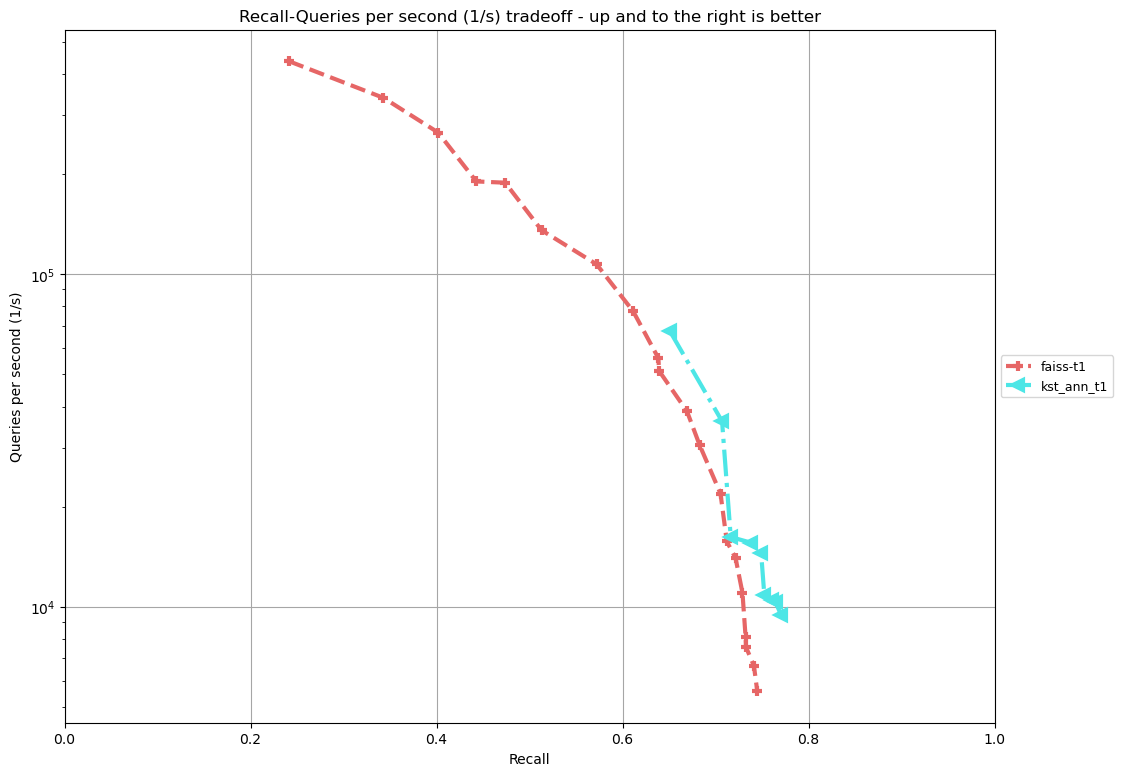
\includegraphics[width=\linewidth]{../t1_t2/results/T1/neurips21/msspacev-1B.png}
      \caption{msspacev-1B}
  \end{subfigure}
  \begin{subfigure}{0.48\textwidth}
    \centering
    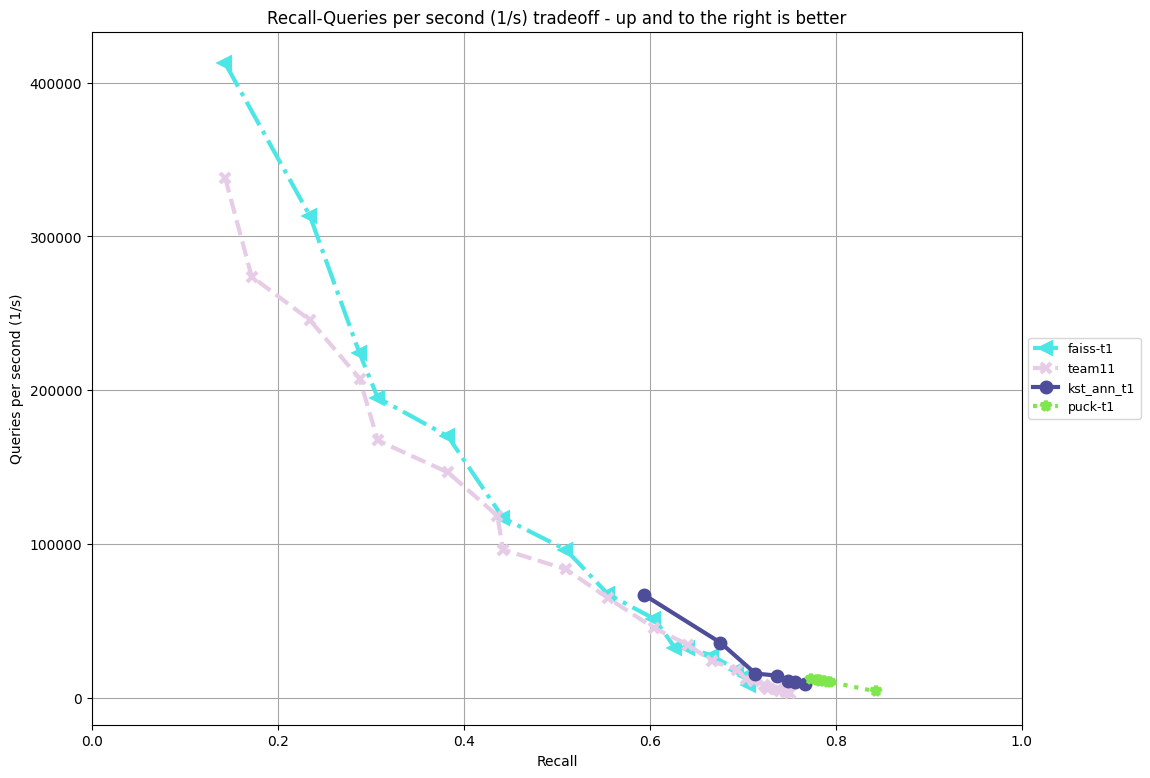
\includegraphics[width=\linewidth]{../t1_t2/results/T1/neurips21/msturing-1B.png}
    \caption{msturing-1B}
  \end{subfigure}
  \begin{subfigure}{0.48\textwidth}
    \centering
    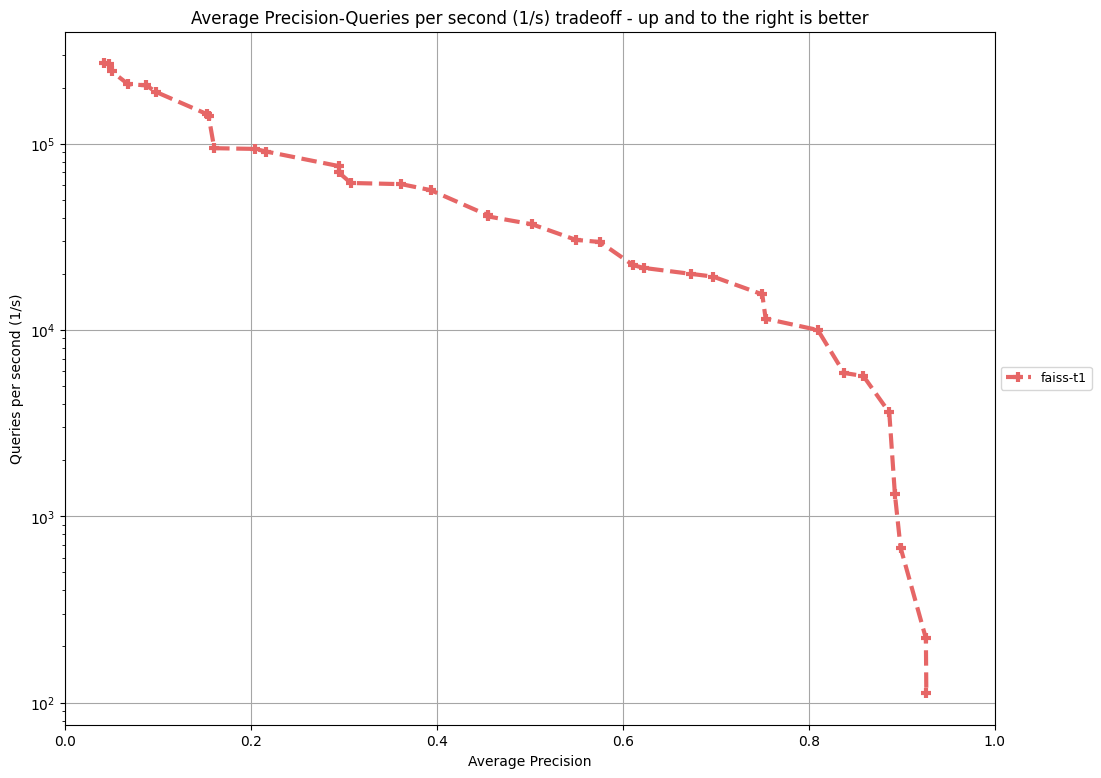
\includegraphics[width=\linewidth]{../t1_t2/results/T1/neurips21/ssnpp-1B.png}
      \caption{ssnpp-1B}
  \end{subfigure}
  \begin{subfigure}{0.48\textwidth}
    \centering
    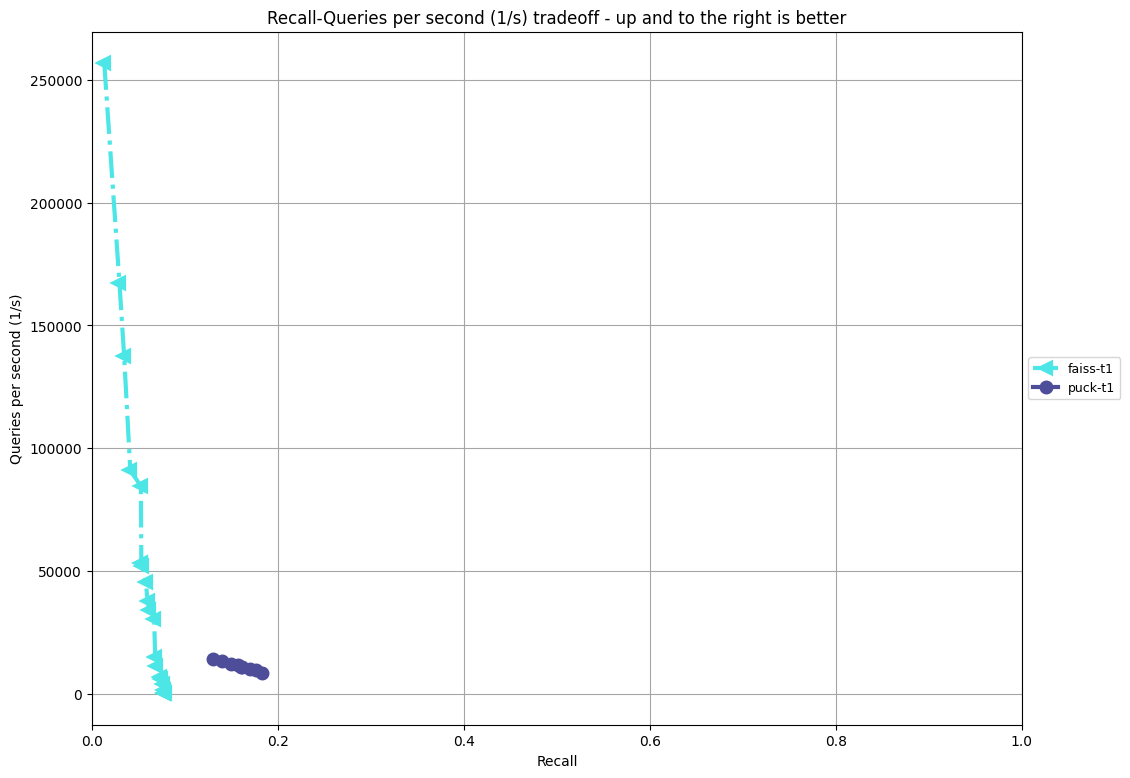
\includegraphics[width=\linewidth]{../t1_t2/results/T1/neurips21/text2image-1B.png}
    \caption{text2image-1B}
  \end{subfigure}
      
  \caption{QPS vs Recall plots for each dataset in Track T1.}
  
\end{figure}

\subsection{Track 2}
\begin{table}
  \caption{Leaderboard for Track T2. Recall achieved at 1500 QPS on Azure Ls8v2 VM with 8 vCPUs.}
  \begin{tabular}{l|c|c|c|c|c|c}
    \hline
    Algorithm & bigann-1B  & deep-1B & msspacev-1B & msturing-1B &   ssnpp-1B  &     text2image-1B \\
    \hline
    baseline &  0.94913 & 0.93706 & 0.90095 & 0.93564 & 0.16274 & 0.48854 \\
    \hline
    \href{https://github.com/harsha-simhadri/big-ann-benchmarks/pull/62}{kota-t2} & 0.950859 & & 0.904001 & 0.939817 & 0.18212 & \\
    \href{https://github.com/harsha-simhadri/big-ann-benchmarks/pull/6}{ngt-t2} & & & & & & \\
    \href{https://github.com/harsha-simhadri/big-ann-benchmarks/pull/70}{bbann} & & & 0.7602 & & 0.88573 & 0.495423 \\
    \hline
     
  \end{tabular}
  
\end{table}



\begin{figure}[ht]
  \begin{subfigure}{0.48\textwidth}
    \centering
    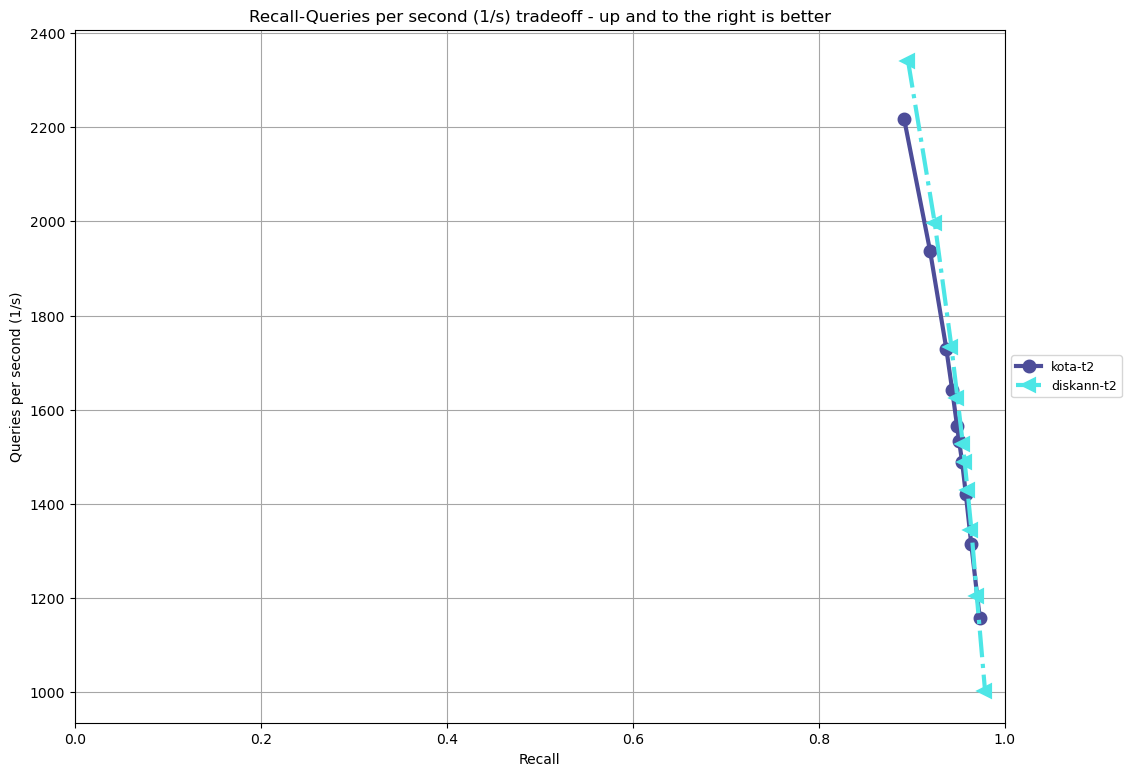
\includegraphics[width=\linewidth]{../t1_t2/results/T2/neurips21/bigann-1B.png}
      \caption{bigann-1B}
  \end{subfigure}
  \begin{subfigure}{0.48\textwidth}
    \centering
    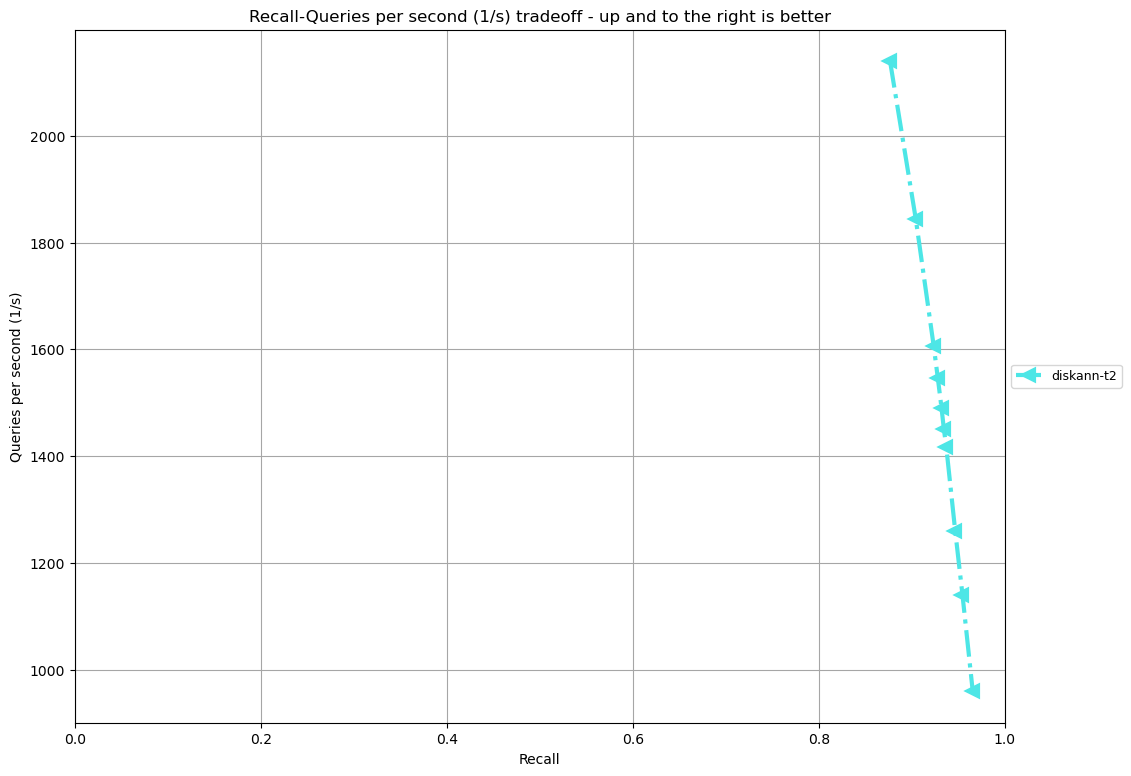
\includegraphics[width=\linewidth]{../t1_t2/results/T2/neurips21/deep-1B.png}
    \caption{deep-1B}
  \end{subfigure}
  \begin{subfigure}{0.48\textwidth}
    \centering
    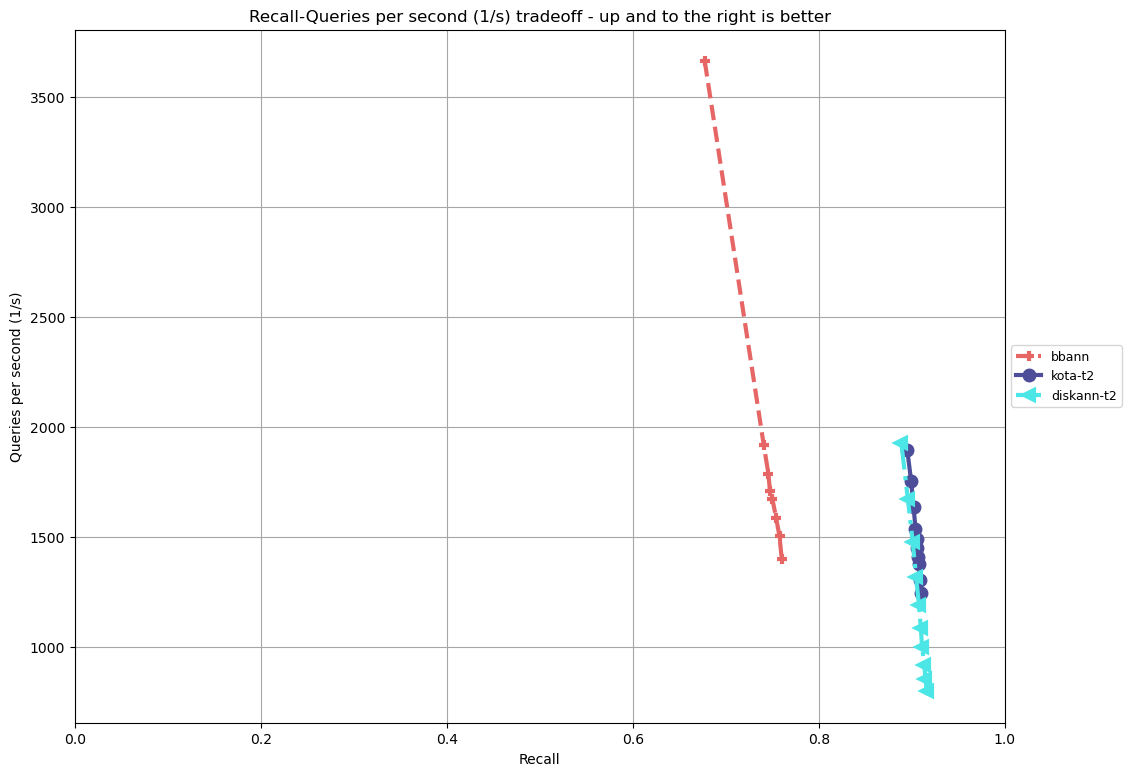
\includegraphics[width=\linewidth]{../t1_t2/results/T2/neurips21/msspacev-1B.png}
      \caption{msspacev-1B}
  \end{subfigure}
  \begin{subfigure}{0.48\textwidth}
    \centering
    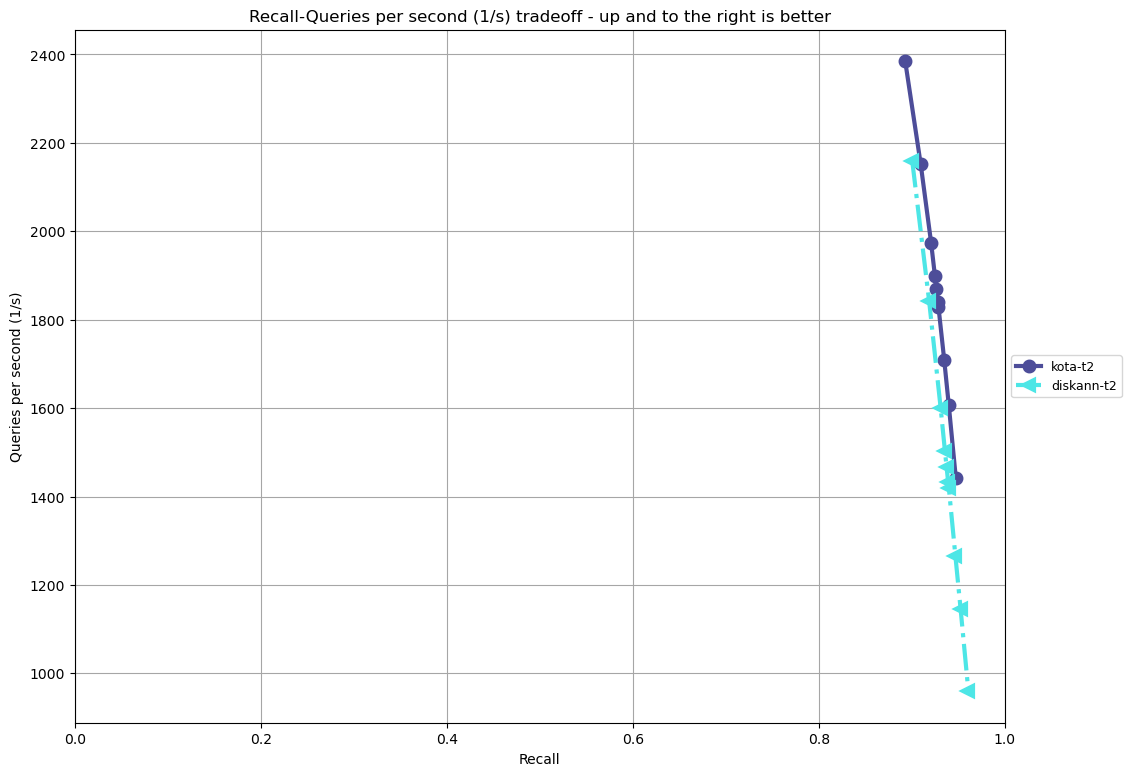
\includegraphics[width=\linewidth]{../t1_t2/results/T2/neurips21/msturing-1B.png}
    \caption{msturing-1B}
  \end{subfigure}
  \begin{subfigure}{0.48\textwidth}
    \centering
    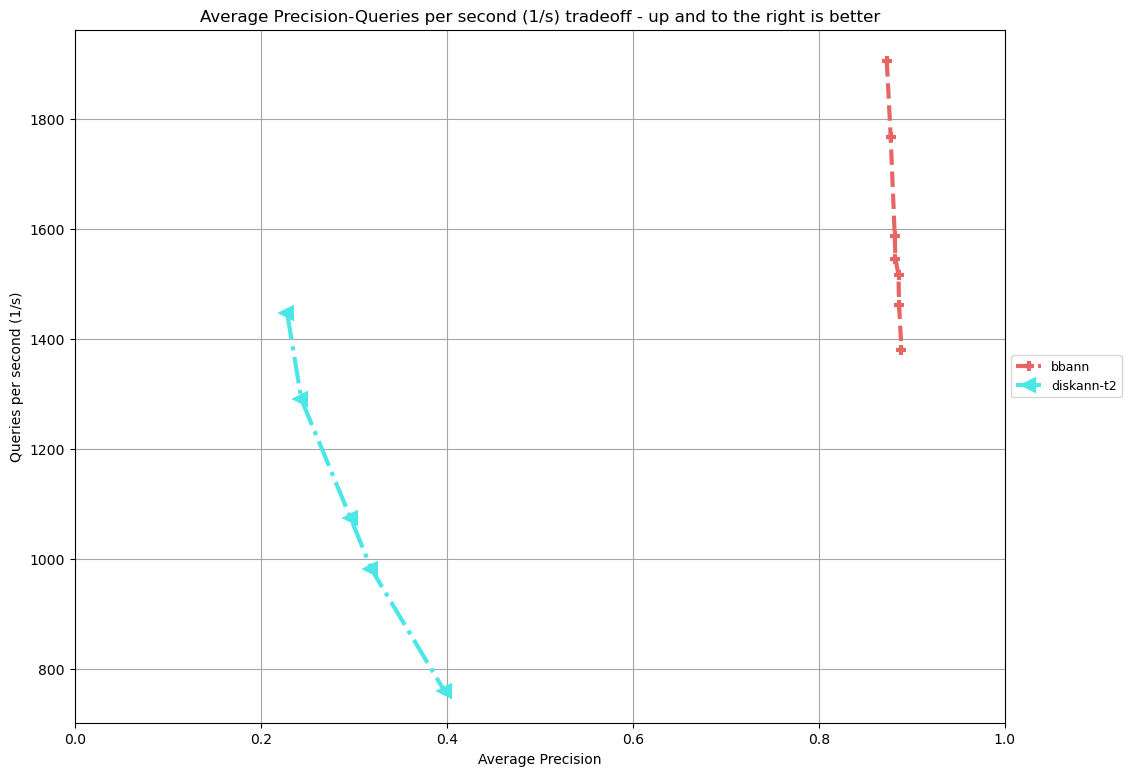
\includegraphics[width=\linewidth]{../t1_t2/results/T2/neurips21/ssnpp-1B.png}
      \caption{ssnpp-1B}
  \end{subfigure}
  \begin{subfigure}{0.48\textwidth}
    \centering
    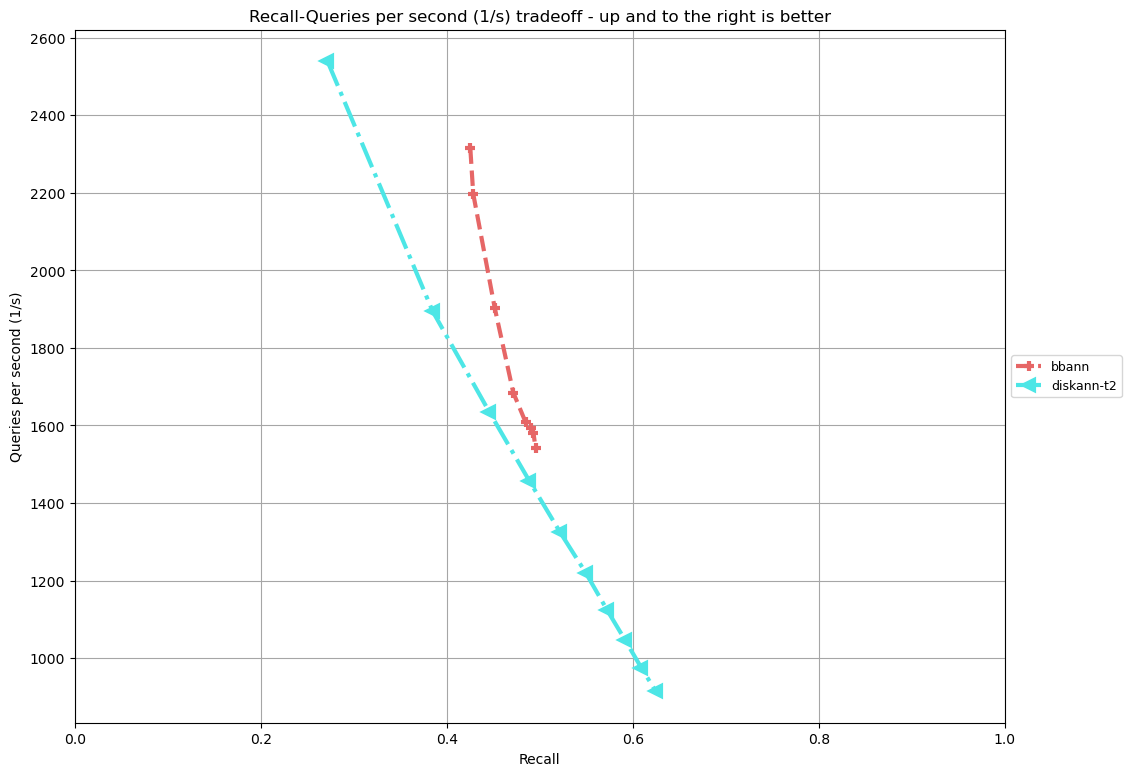
\includegraphics[width=\linewidth]{../t1_t2/results/T2/neurips21/text2image-1B.png}
    \caption{text2image-1B}
  \end{subfigure}
      
  \caption{QPS vs Recall plots for each dataset in Track T2::.}

\end{figure}

\subsection{Track 3}
